\chapter{Principle of the FFT code}
\pagestyle{headings}

In this chapter, we detail the two main steps used to propagate an electric field in a Fabry-Perot cavity. Firstly we will understand how the propagation of any arbitrary electric fields can be simulated using a Fourier transform. And secondly, we will see how any wavefront distortions encountered by the electric fields can be included in the numerical simulations. Whenever possible some simple Matlab codes are presented to show the numerical implementation of the algorithm. For clarity, the snippets of code are \textbf{not} optimised.

\section{Why OSCAR ?}

OSCAR is a FFT code which is able to simulate Fabry Perot cavities with arbitrary mirror profiles. One of the key features of OSCAR is the possibility to easily modify the code to suit the user purpose. For this reason, OSCAR is written with the Matlab language, one can import/export files (mirror maps or cavity eigenmodes profile for example), create a ring cavity, create batch file or plot 2D optical field with little programming skill\footnote{The code  can also be useable with the free Matlab-alternatives such as Sci-Lab or Octave with only minor modifications. Even a minimal Python version also exists.}. The fact that I encourage everyone to understand the code of OSCAR in details and to also modify it, is the main reason for this lengthy manual.

\subsection{Origin of OSCAR}

I started writing and using OSCAR during my PhD where I had to simulate the effects of thermal lensing in high optical power cavities. Wavefront distortions induced by the optical absorption have seldom pure spherical profiles, which means it is delicate to quantify thermal lensing effects with modal expansion code (but still possible).
To simulate the effects of the optical absorption on the mirror, I was using the FEM package Ansys which can calculate the temperature distribution inside the mirror substrate or the surface deformations due to the absorption of a Gaussian beam. From the Ansys results, it is straight forward to calculate the wavefront distortion induced by thermal lensing. However, at this stage, I was facing a problem, how can I estimate the effects of the thermal lens if it has to be inserted in a Fabry-Perot cavity ? how much the circulating power will decrease ? Will the cavity optical modes keep their Gaussian profiles ? I needed an optical simulation tool which can be used with any arbitrary mirror profile. OSCAR was born. For the inquisitive reader, the name OSCAR is the acronym of Optical Simulation Containing Ansys Results.

The first version of OSCAR was written with the software IGOR. This code was then translated to Matlab and used to calculate diffraction losses by my UWA colleague Pablo Barriga. Finally, I re-wrote and optimised the Matlab code to substantially decrease the OSCAR computational time. During the year 2011, OSCAR was totally revamped using the Oriented Object capability of Matlab giving rise to the Version 3.0.

\subsection{Which results could I get from OSCAR ?}

OSCAR is a versatile tool to simulate Fabry Perot cavities. The following is a (non-exhaustive) list of the results which can be obtained with OSCAR:
\begin{itemize}
  \item calculate the Gouy phase shift between higher order optical modes. It may be useful for flat beams for example, where no analytical calculations of the Gouy phase shift has been derived yet (as far as I know)
  \item calculate the coupling loss between the input beam and the cavity eigenmodes in case mode mismatching
  \item calculate the circulating beam (intensity and profile) inside the cavity, which may be different from the eigenmodes if the cavity has a low finesse
  \item calculate diffraction loss and eigenmodes of cavity for arbitrary mirror profiles
  \item calculate the effects of imperfect optics, due to the micro-roughness of the coating surface or thermal lens inside the substrate of the mirrors.
\end{itemize}

Even more complicated configuration could also be simulated such as dual recycled Michelson with Fabry-Perot arm cavities (topology of advanced laser gravitational wave detectors). However the code is more complex and lacking exhaustive documentation, but it is available on demand.

\subsection{What OSCAR is not for}

OSCAR is designed to simulate anything which can be derived from the steady state, classical, optical field circulating inside a Fabry-Perot cavity. It means OSCAR does not take into account radiation pressure or quantum effect (no shot noise calculations).

\section{Propagation of an optical field}
\label{sec1.2}

In this section we will see how it is possible to propagate a coherent electric field, i.e. a laser beam, with the help of the Fourier transform. The principle of the FFT optical propagation code is similar to the Fourier transformation method used to calculate the response of a linear system to an arbitrary function $f_i(t)$. The function $f_i(t)$ is expressed as a continuous superposition of harmonic functions of different frequencies $\nu$:
\begin{equation}
 f_i(t) = \int_{-\infty}^{\infty} \widetilde{f_i}(\nu) \exp(2\pi j \nu t) d\nu
\label{eq1:four}
\end{equation}

\noindent Where $\widetilde{f_i}$ is the Fourier transform of the function $f_i$. The function $ t\rightarrow \exp(2\pi j \nu t)$ is the harmonic function of frequency $\nu$. These are the basic functions used to expand $f_i$. If the response of the system is known for each elementary harmonic function $\exp(2\pi j \nu t)$, the response of the system to the input $f_i$ can be derived using three steps. First step, the function $f_i$ is expanded in the sum of basic harmonic functions by doing a Fourier transformation. Second step the response of the system to each harmonic function is calculated. This is done simply by a multiplication in the frequency domain. Finally, third step, the output of the system to the input $f_i$ is derived by doing the inverse Fourier transformation of the output harmonic functions (step similar to the equation \ref{eq1:four}).\\

The FFT optical propagation code follows exactly the principle described in the previous paragraph. In this case the elementary functions are plane waves of different spatial frequencies.

\subsection{Propagation of a plane wave}

We can first understand how to propagate of an elementary plane wave $u$ through free space. At $z = 0$, $u$ can be simply written:

\begin{equation}
u(x,y,0) = \exp(-j k_x x - j k_y y)
\label{eq1:uel}
\end{equation}

\noindent with $k_{x/y}$ the propagation constant along the $x/y$ axis. Equation (\ref{eq1:uel}) can also be written:
\begin{equation}
u(x,y,0) = \exp(-j 2 \pi (\nu_x x + \nu_y y)) \mbox{ with } \nu_x = k_x/(2 \pi) \mbox{ and } \nu_y = k_y/(2 \pi)
\label{eq1:uel2}
\end{equation}

If $u$ is written as shown in equation (\ref{eq1:uel2}), it is easy to recognise $u$ as a harmonic function of two variables $(x,y)$ with respective spatial frequencies \footnote{The term spatial frequency $\nu$ must be understood as the number of wavelength per unit of length $\nu = 1/\lambda = k / 2\pi$} $(\nu_x,\nu_y)$. If we propagate $u$ along the z axis over a distance d:
\begin{equation}
u(x,y,d) = \exp(-j k_x x - j k_y y - j k_z d)
\label{eq1:uel3}
\end{equation}

\begin{figure}
\begin{center}
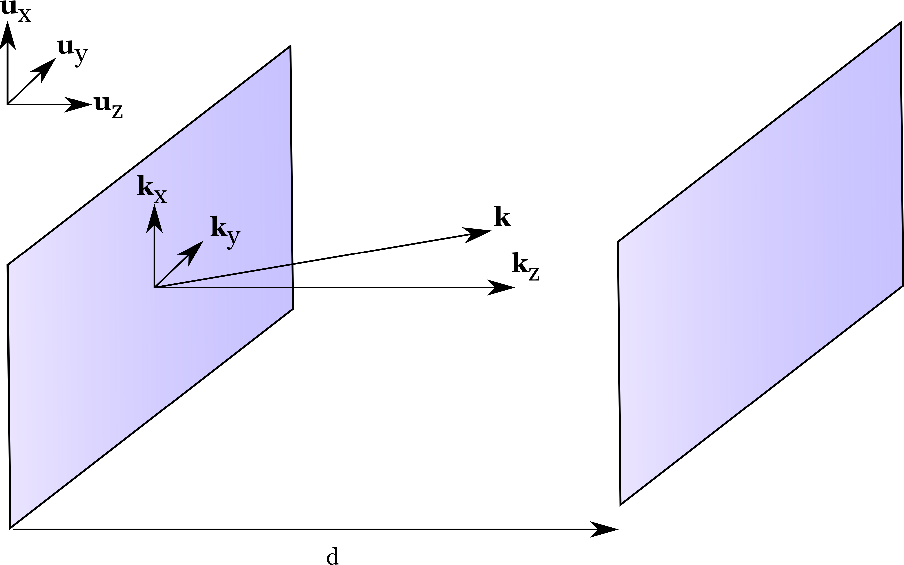
\includegraphics[width = 0.80\textwidth]{Planewave.pdf}
\end{center}
\caption{\label{fig1:plane} Propagation of a plane wave along the z axis.}
\end{figure}


\noindent with $k =  (k_x^2 + k_y^2 + k_z^2)^{\frac{1}{2}} = 2 \pi / \lambda $. If we suppose the wave to be traveling in a direction close to the z axis (paraxial approximation) as shown in figure \ref{fig1:plane}, $k_z \gg k_x$ and $k_z \gg k_y$, then $k_z$ can be written as:
\begin{eqnarray}
k_z = (k^2 - k_x^2 - k_y^2)^{\frac{1}{2}} & \simeq & k - \frac{(k_x^2 + k_y^2)}{2 k } \label{eq4:uel4a}\\
& \simeq & k - \lambda \pi (\nu_x^2 + \nu_y^2)
\label{eq1:uel4}
\end{eqnarray}

\noindent So we can rewrite equation (\ref{eq1:uel3}) as:
\begin{equation}
u(x,y,d) = u(x,y,0) \exp(-j (k - \lambda \pi (\nu_x^2 + \nu_y^2))d)
\label{eq1:uel5}
\end{equation}

The equation (\ref{eq1:uel5}) is the foundation of the FFT propagation code. It tells us that the propagation of a plane wave along the z axis over a distance $d$ can simply be represented by a phase shift. The function $ d\rightarrow \exp(-j (k - \lambda \pi (\nu_x^2 + \nu_y^2))d)$ could also be seen as the propagation operator for an input plane wave traveling a distance $d$ under the paraxial approximation. The term $\exp(-j (k d))$ represents the phase shift of a plane wave propagating along the z axis and the term $ \exp (j \lambda \pi (\nu_x^2 + \nu_y^2)d)$ adds a phase correction to take into account the fact that the wave propagates with a small angle with respect to the z axis\footnote{The angle $\theta_x$ between the direction of propagation and the x axis is $\theta_x = sin^{-1}(k_x/k)$. In the case of small angles, it is simply $\theta_x = \lambda \nu_x$}.\\


We noticed in equation (\ref{eq1:uel2}), that the elementary plan wave $u(x,y,0)$ can also be seen an harmonic function with spatial frequency $\nu_x$ and $\nu_y$. To keep the analogy developed in the introduction of this chapter with the classical time domain Fourier transform, the plane wave is equivalent to the elementary harmonic function $t\rightarrow \exp(2\pi j \nu t)$ of frequency $\nu$. Since we know how to propagate a plane wave, we understand now how it may be possible to propagate any arbitrary field if we can manage to expand it as a superposition of elementary plane waves.

\subsection{Propagation of an arbitrary field}

Equation (\ref{eq1:uel5}) tells us how to propagate a plane wave. So to propagate any arbitrary electric fields $E$, we need to know how to expand the electric field onto the set of plane waves $\exp(-j 2 \pi (\nu_x x + \nu_y y))$. We would like to find $\widetilde{E}(\nu_x,\nu_y)$ such as:

\begin{equation}
 E(x,y) = \int_{-\infty}^{\infty} \int_{-\infty}^{\infty} \widetilde{E}(\nu_x,\nu_y) \exp(-j 2\pi (\nu_x x + \nu_y y)) d\nu_x d\nu_y
\label{eq4:uel6}
\end{equation}

With $\widetilde{E}(\nu_x,\nu_y)$ the complex amplitude of the component of the field $E$ with spatial frequency $(\nu_x,\nu_y)$. We recognise equation (\ref{eq4:uel6}) as an inverse 2D Fourier transform\footnote{In fact, if we respect the convention found in signal processing technique, equation (\ref{eq4:uel6}) is not an inverse Fourier transform but a Fourier transform\cite{Sig_proc}. It is not tragic, since we will stay consistent with the convention presented here.}. Using the properties of the Fourier transform\cite{Fourier_trans} we deduce the expression for $\widetilde{E}(\nu_x,\nu_y)$:

\begin{equation}
  \widetilde{E}(\nu_x,\nu_y) = \int_{-\infty}^{\infty} \int_{-\infty}^{\infty} E(x,y) \exp(j 2\pi (\nu_x x + \nu_y y)) dx dy
\label{eq4:uel7}
\end{equation}

Combining equations (\ref{eq1:uel5}), (\ref{eq4:uel6}) and (\ref{eq4:uel7}) , we know how to propagate in free space a transverse electric field $E$ from $z = 0$ to $z = d$. To calculate the resulting field after the propagation, three steps are required:
\begin{enumerate}

\item Decomposition of the field $E(x,y,0)$ into a sum of elementary plane waves. Mathematically, this step represents a 2D Fourier transformation.

\begin{equation}
 \widetilde{E}(\nu_x,\nu_y,0) = \int_{-\infty}^{\infty} \int_{-\infty}^{\infty} E(x,y,0) \exp(j 2\pi (\nu_x x + \nu_y y)) dx dy
\label{eq1:uel10}
\end{equation}

\item Propagation of each plane waves, which is equivalent of adding a phase shift in the frequency domain.


\begin{equation}
 \widetilde{E}(\nu_x,\nu_y,d) =  \widetilde{E}(\nu_x,\nu_y,0) \exp(-j (k - \lambda \pi (\nu_x^2 + \nu_y^2))d)
\label{eq1:uel11}
\end{equation}

\item Recomposition of the electric field from the propagated plane waves. This step is in fact an inverse Fourier transformation.

\begin{equation}
 E(x,y,d) = \int_{-\infty}^{\infty} \int_{-\infty}^{\infty}  \widetilde{E}(\nu_x,\nu_y,d) \exp(- j 2\pi (\nu_x x + \nu_y y)) d\nu_x d\nu_y
\label{eq1:uel12}
\end{equation}
\end{enumerate}


\subsection{My first Matlab FFT code}

There is an essential point to realize before implementing the three analytical steps described in the previous section. The computer does not deal with continuous electrical fields which means all the data fields have to be discretized. For example the amplitude of a Gaussian beam will be represented by a square matrix (called also grid later), each points of the matrix (called also pixel for convenience) will represent the amplitude of the Gaussian beam at a defined location. A 2D plot of such a matrix is shown in the top left corner of the figure \ref{fig1:FFT}.

Practically, the discretization process is governed by the choice of 2 parameters: the physical size represented by the matrix and the number of points in the matrix. For example, to discretize a laser beam with a beam radius of 1~cm we can use a matrix of size $128 \times 128$ representing an area of 10~cm by 10~cm. This example can be implemented in Matlab in a straight forward way as shown in the listing \ref{lis1:start1}.

\begin{lstlisting}[float=tp,caption=Discretization of a Gaussian beam\label{lis1:start1},frame=lines]
Grid.Num_point = 128;                                % Number of point in one side the grid
Grid.Length = 0.10;                                  % Physical dimension of the grid in meter
Grid.step = Grid.Length/Grid.Num_point;              % Physical size of one pixel of the grid

Grid.vector = 1:Grid.Num_point;                      % Grid.vector = 1 2 3 ... Grid.Num_point
% Calculate the spatial scale used for each pixel:
Grid.axis = -Grid.Length/2 + Grid.step/2 + (Grid.vector-1)*Grid.step;

Field.Gaussian = zeros(Grid.Num_point,Grid.Num_point,'double');
Laser.amplitude = 1;                                 % Arbitrary amplitude
Laser.waist = 0.01;                                  % waist of the laser beam in meter

% Fill the matrix representing the (real) Gaussian beam:
for m = 1:Grid.Num_point
    for n = 1:Grid.Num_point
        Field.Gaussian(m,n) = Laser.amplitude * exp(-(Grid.axis(m)^2+Grid.axis(n)^2)/Laser.waist^2);
    end
end

\end{lstlisting}

If the scale of the matrix (called \emph{Grid.axis} in the listing \ref{lis1:start1}) representing the amplitude distribution is easy to understand, a more delicate point is the scaling of the Fourier transform of the input beam. This scaling of the spatial frequency is required since we need to know the spatial frequency represented by each pixel of the discrete Fourier transform of the Gaussian beam. Concretely we need to know the discrete values of $\nu_x,\nu_y$ from equation \ref{eq1:uel10}.

First thing to understand is that the discrete Fourier transform of a 2D complex matrix is also a 2D complex matrix with the same dimensions \cite{Fourier2D}. The low spatial frequencies are located in the middle of the matrix and the high spatial frequencies on the edge. Typically if the original matrix has for dimensions $N \times N$, the spatial frequency 0 (the average component) is located at the index $(N/2+1,N/2+1)$\footnote{In fact the FFT algorithm returns the Fourier transform of the input matrix with the low spatial frequency spread at the four corners of the matrix. However for a better readability, the low frequency are then shifted back to the center of the matrix.}. Meanwhile, the frequency separation $\Delta \nu$ between 2 adjacent pixels of the Fourier matrix is:

\begin{equation}
 \Delta \nu = \frac{1}{Grid.Length} =\frac{1}{N \times Grid.step}
\end{equation}

With \emph{Grid.Length} and \emph{Grid.step} the variables defined in the listing \ref{lis1:start1}. So the minimal (negative) spatial frequency calculated is $- N/2 *\Delta \nu$ often called the Nyquist frequency and the maximal spatial frequency is $(N/2-1) *\Delta \nu$. An example for the frequency scale of the Fourier transform of the matrix is presented in the top right plot of the figure \ref{fig1:FFT}.

Special attention must be taken to understand the vertical and horizontal scales in the figure \ref{fig1:FFT}. The numbers written for the scales are in fact the value of the scale between 2 pixels as it can be seen by zooming on the ticks. So for example to know what is the spatial frequency of the first top row (horizontal line) of the Fourier matrix on the top right plot which represents the maximal spatial frequency, we have to take the average of the top two ticks. So the maximal spatial frequency is $1/2*(96.875 + 90.625) = 93.75 \textrm{m}^{-1}$, which is as expected equal to $(N/2-1) *\Delta \nu = 15/0.16 = 93.75 $\\


% saved figure files from IGOR size 17cm*17cm
% Margin 3,3,0.49,0.49
% Officia Sans IT 14

\begin{figure}
\begin{center}
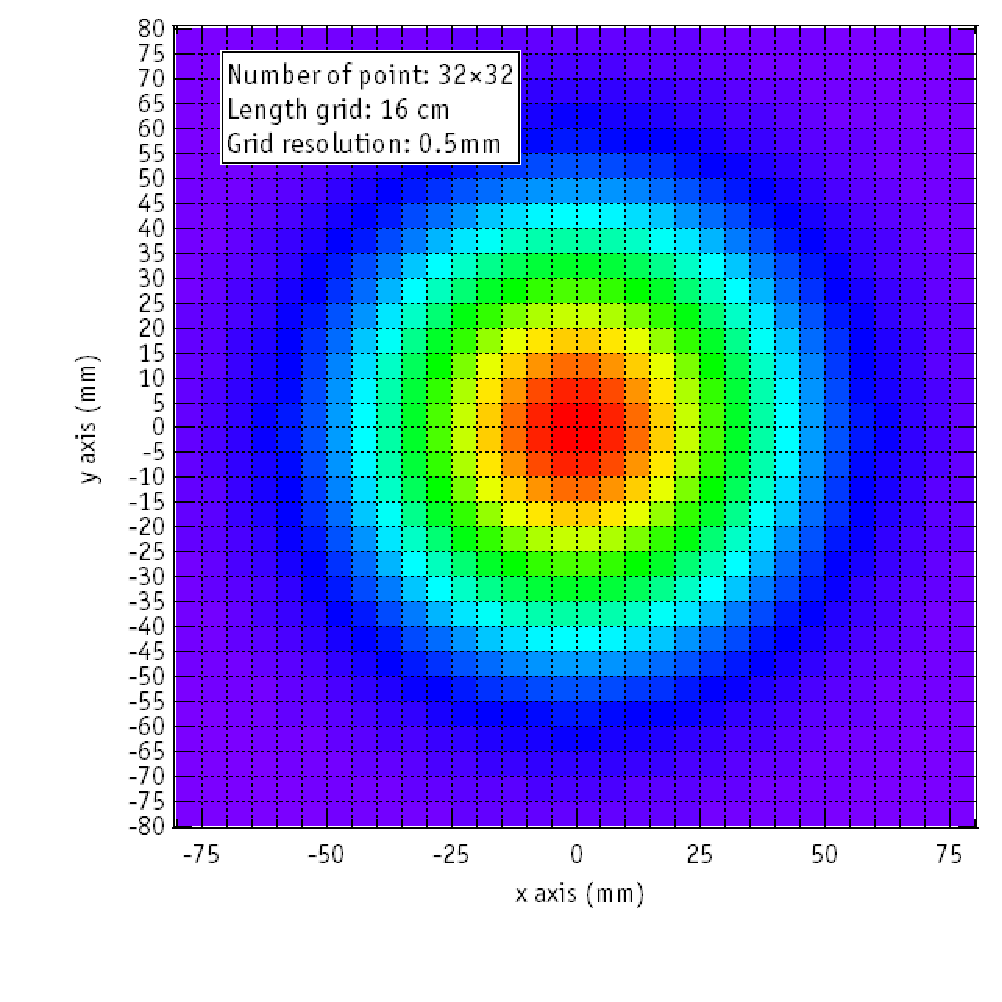
\includegraphics[width = 0.45\textwidth]{T1_FFT1a.pdf}\hfill
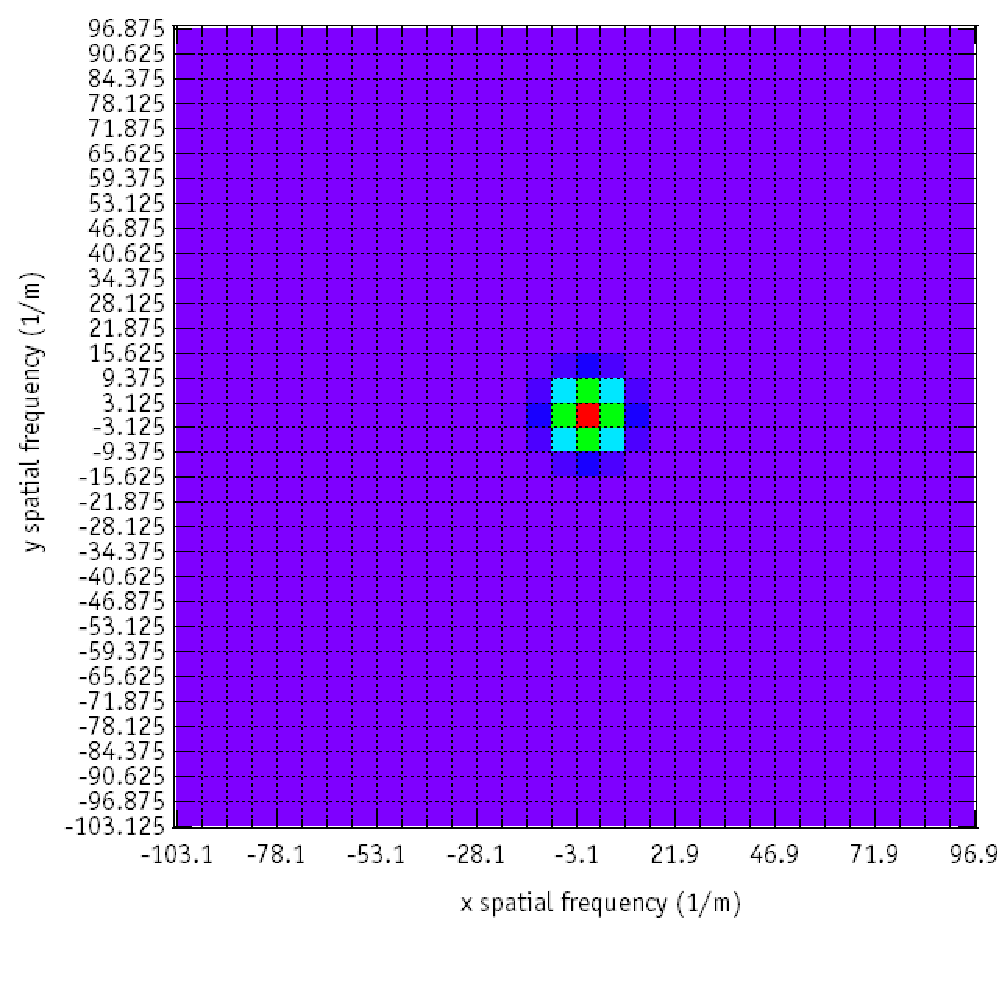
\includegraphics[width = 0.45\textwidth]{T1_FFT1b.pdf}

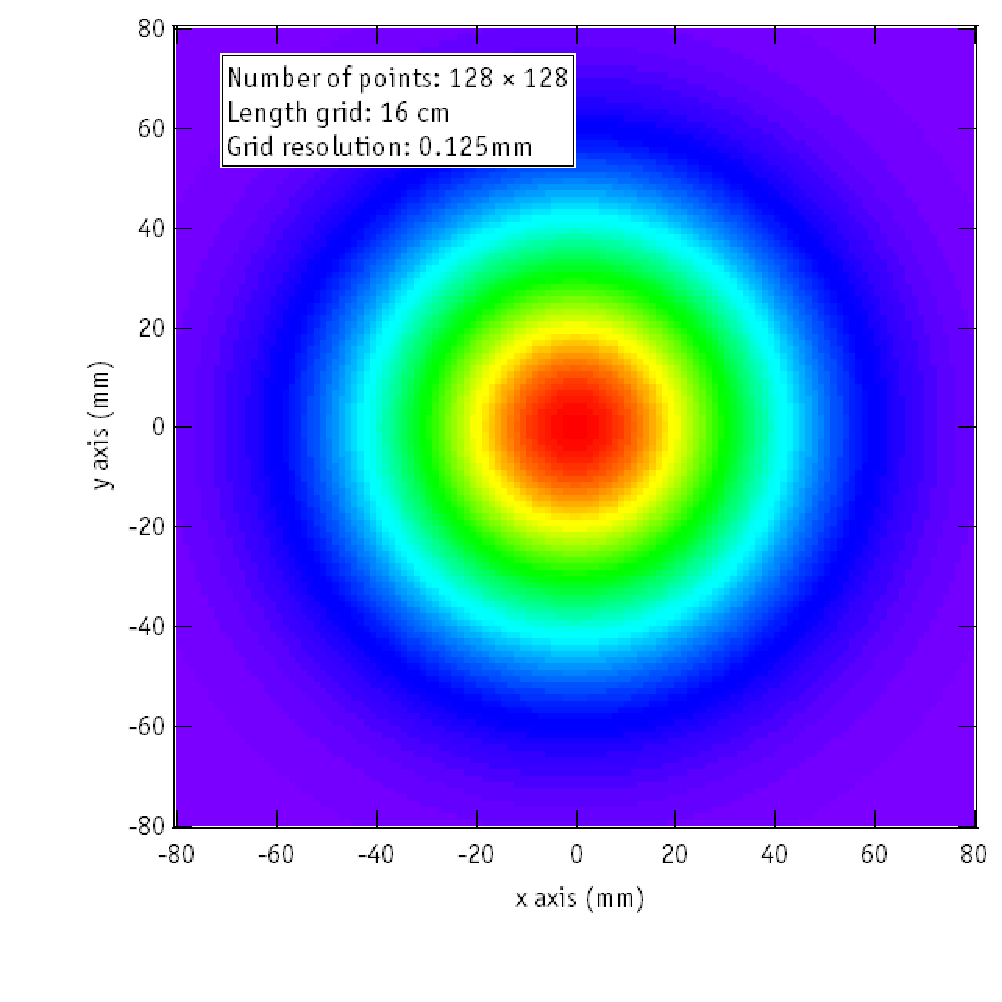
\includegraphics[width = 0.45\textwidth]{T1_FFT2a.pdf}\hfill
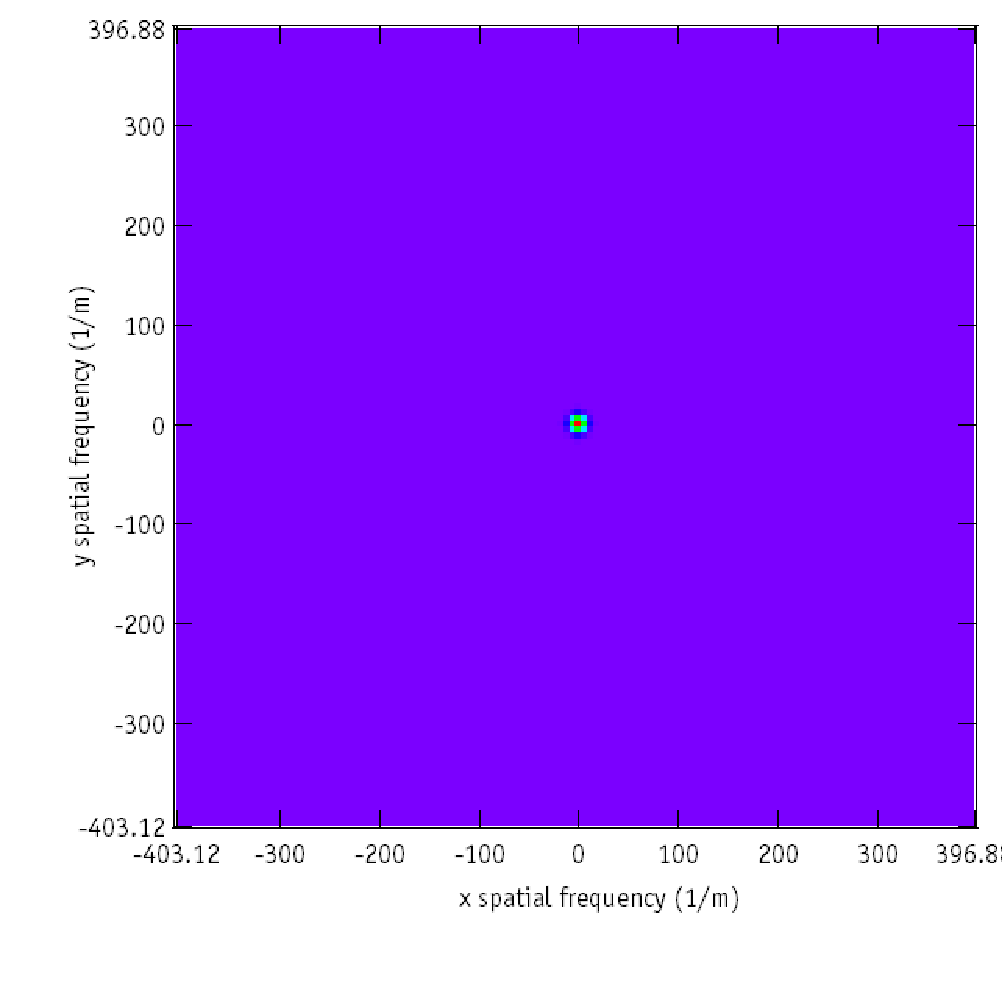
\includegraphics[width = 0.45\textwidth]{T1_FFT2b.pdf}

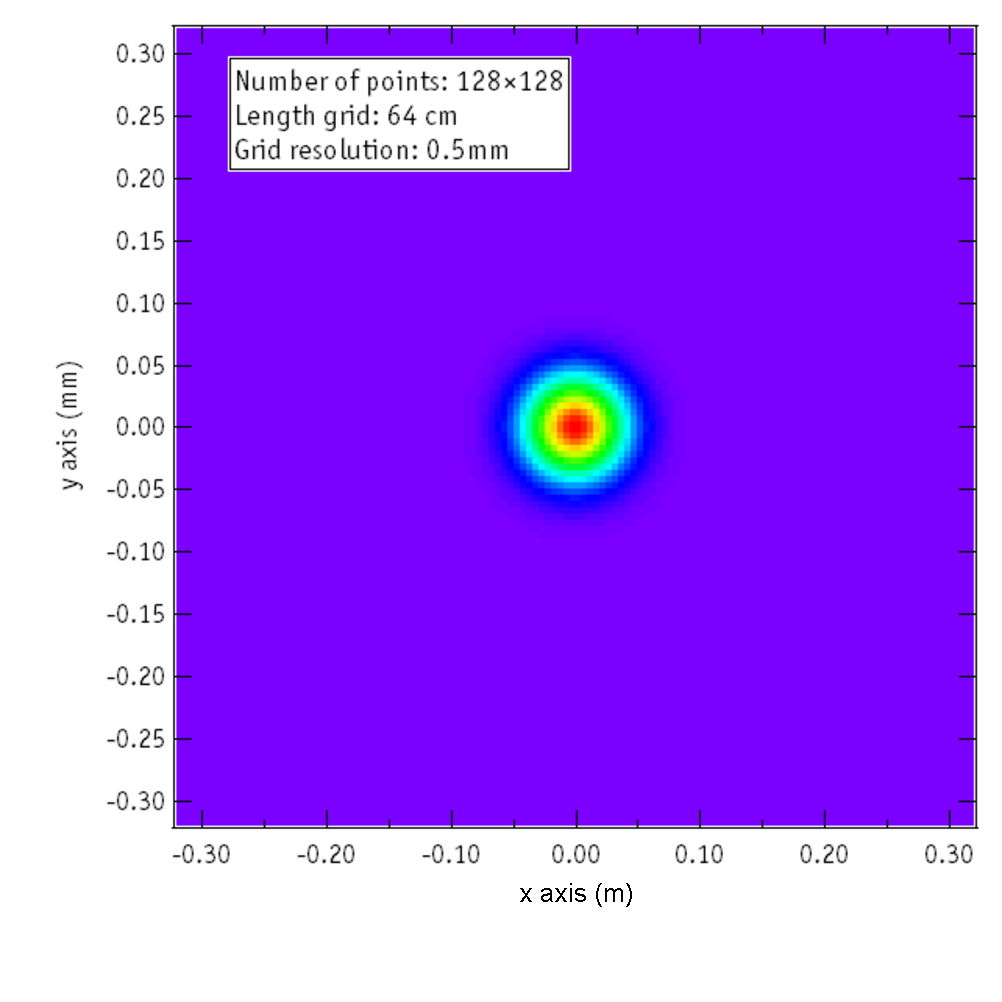
\includegraphics[width = 0.45\textwidth]{T1_FFT3a.pdf}\hfill
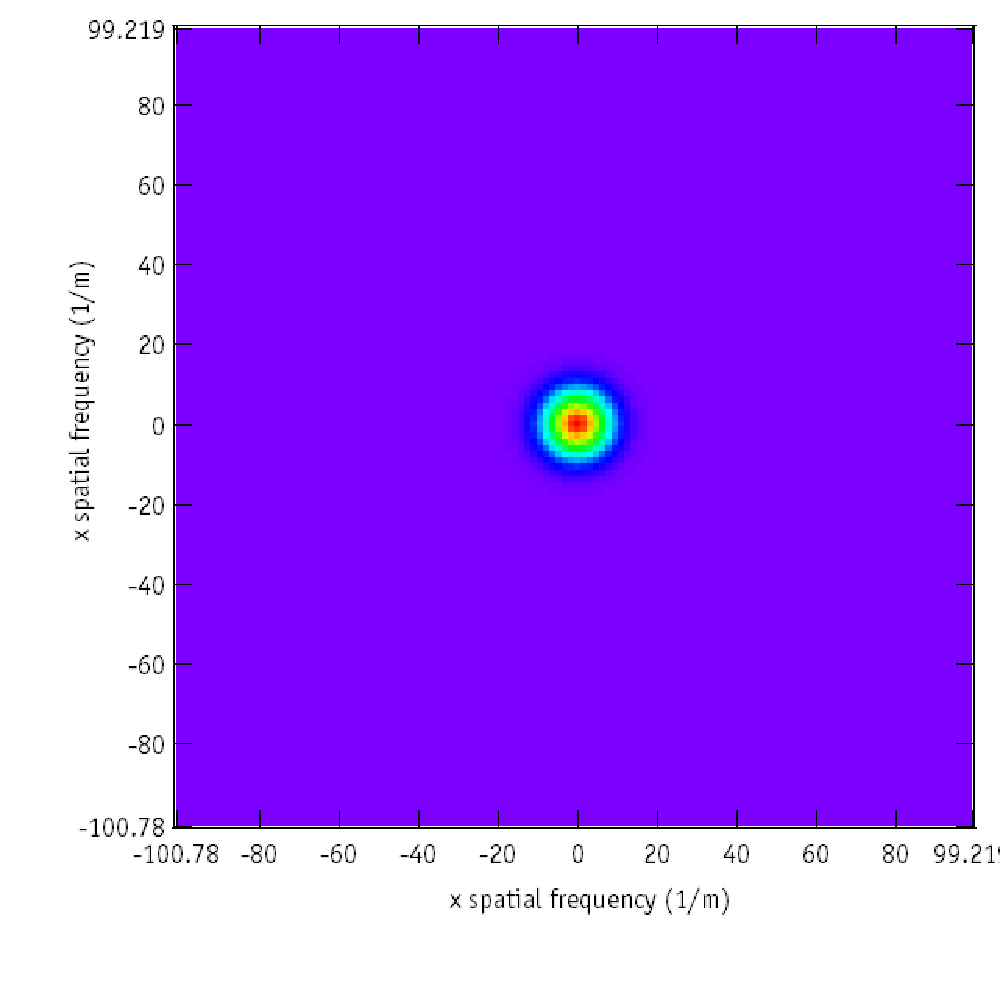
\includegraphics[width = 0.45\textwidth]{T1_FFT3b.pdf}

\end{center}
\vspace*{-0.8cm}
\caption{\label{fig1:FFT} Example of the influence of the physical size of the grid and the number of points used for the representation of a Gaussian beam (left column) and its Fourier transform (right column). As expected intuitively, to have a proper representation of both the Gaussian beam and its Fourier transform it is essential to have simultaneously a large space window (parameter: \textsl{Grid.Length}) and a large number of points (parameter: \textsl{Grid.Num\_point}). For this example the waist of the laser beam is 4~cm. }
\end{figure}

One natural question we could ask is what is the good size of the grid ? The size of the grid must be large enough to represent faithfully the Gaussian beam, no substantial energy from the beam must lay outside the grid. So the dimension of the grid must be \emph{at least} 3-4 times bigger than the biggest beam diameter encountered. A large grid size is also important to sample properly the low special frequency as shown at the bottom of figure \ref{fig1:FFT}. Remarkably even if the laser beam radius increased as the beam propagates from its waist, the amplitude of the Fourier transform is constant along the propagation. Indeed the propagation as shown in equation \ref{eq1:uel11} is simply represented by a phase shift in the Fourier domain.\\

After the physical size of the grid has been chosen, the second important parameter to be decided is the number of points in the grid. Because of the way the discrete Fourier transform is calculated in the FFT algorithm, it is strongly recommended to choose the number of points for the side of the matrix to be a power of 2. Usually a good compromise between speed and accuracy is given for N =64,128 or 256. The influence of the number of points on the accuracy of the results can (and should) always be checked by doing the same simulations with different mesh of the grid.\\

The size of the grid divided by the number of pixels is the dimension represented by one pixel, in other word the resolution of the grid (variable \emph{Grid.step}). Of course, the resolution of the grid must match the size of the physical feature we would like to simulate. For example it is useless to try to simulate the effect of features having a size 1~mm in a mirror map with a grid resolution of 1~cm.\\


We just saw how a square matrix can be used to represent a discrete electric field, so now we can try to simulate its propagation it using the 3 consecutive steps described by equations (\ref{eq1:uel10}), (\ref{eq1:uel11}) and (\ref{eq1:uel12}). During the second step, the Fourier transform of the electric field is multiply by a complex number depending of the distance of propagation and also the spatial frequency. Practically this multiplication is achieved by multiplying pixel by pixel 2 matrices: the Fourier transform matrix with a propagation matrix. The propagation matrix is usually defined before hand and only once since it will be used repeatedly as we will see later in section \ref{sec1.4}. The matlab code at the core of the FFT code is presented in the listing \ref{lis1:start2}, it is the direct sequel from the previous listing where we defined the matrix used to represent the electric field.\\

%\vspace*{1cm}

\begin{lstlisting}[float=tp,caption=The code used to propagate the matrix Field.Start \label{lis1:start2},frame=lines]

% Distance of propagation in meter
Distance_prop = 100;

% Spatial frequency of the pixels in the Fourier space
Grid.axis_fft = -1/(2*Grid.step) + (Grid.vector-1)*1/(Grid.Num_point*Grid.step);

% Define the propagation matrix

Mat_propagation = zeros(Grid.Num_point,Grid.Num_point,'double');

for m = 1:Grid.Num_point
    for n = 1:Grid.Num_point

        Mat_propagation(m,n) = exp(i*(-Laser.k_prop*Distance_prop + ...
            pi*Laser.lambda*(Grid.axis_fft(m)^2 + Grid.axis_fft(n).^2)*Distance_prop));

    end
end

%------------------ Propagate the field ---------------------------

Field.Fourier = fftshift(fft2(Field.Start));       % Do the Fourier transform of the input field
Field.Fourier = Field.Fourier .* Mat_propagation;  % Do the propagation in the frequency domain
Field.End = ifft2(ifftshift(Field.Fourier));       % Do the inverse Fourier transform

% As a result Field.End represents Field.Start propagated over 100 meters
\end{lstlisting}


The propagation of an electric field using a FFT code is an extremely powerful tool. With the FFT code we can propagate any arbitrary profile of the laser beam, not only the beams from the usual Hermite Gaussian set. Such an example is presented in figure \ref{fig4:FFTsquare}. The code used to produce these two plots is given with the OSCAR distribution, the name of the Matlab script is \textcolor{blue}{My\_First\_FFT\_code.m}. The initial field is a theoretical square of uniform amplitude (left plot). The resulting field after the propagation in free space over 100~m is shown in the right plot. A similar result could have been obtained based on the propagation of Hermite Gaussian modes. However to have an accurate representation of the initial field, a very large number of the higher order modes must have been taken into account which requires large amount of computer processing power. The field is discretise on a 1024 $\times$ 1024 matrix. The physical size of the grid is 16~cm $\times$ 16~cm.\\


% 1.5,2,3,0.5
% 14cm 11cm

\begin{figure}
\begin{center}
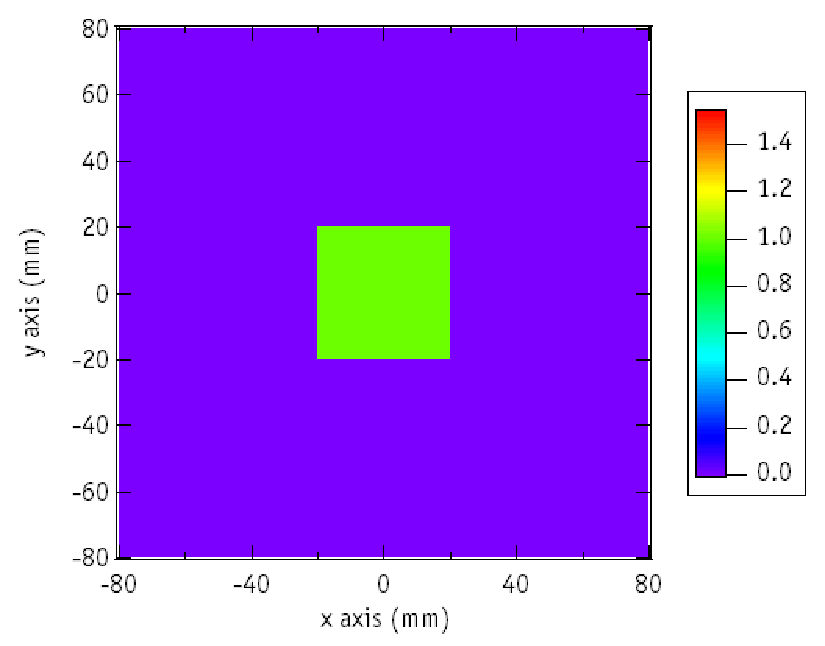
\includegraphics[width = 0.5\textwidth]{T1_Beam_before.pdf}\hfill
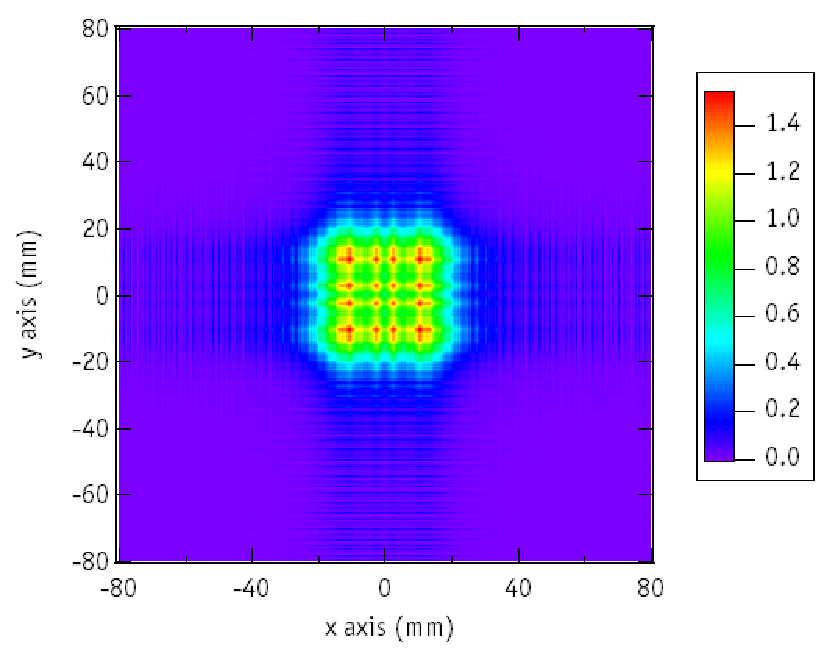
\includegraphics[width = 0.5\textwidth]{T1_Beam_after.pdf}
\end{center}
\caption{\label{fig4:FFTsquare} Propagation of an uniform square of light using our FFT propagation code. The initial square light field is presented on the left plot. The field resulting from the propagation of the initial field over 100~m is shown on the right plot. Structures similar to the Hermitte Gaussian modes begin to emerge when the square field propagates in free space.}
\end{figure}

We arrive now at the end of this section which is dedicated to understand how we can numerically simulate the propagation of an arbitrary laser beam. However having a code only capable to propagate a beam is seldom useful. We are usually more interested to simulate real optical system with mirrors, aperture and imperfect optics. How to include optics in the code is the subject of the next section.\\

\clearpage


\section{Adding realistic optics}
\label{sec1.3}

It is time now to introduce in our simulation two essential optical components: mirrors and lenses. Theses components alter the beam wavefront radius of curvature and so are used for beam shaping (in clear: they make the laser beam smaller or bigger). This can be easily implemented in OSCAR as we will discover in the following paragraphs.



\subsection{Arbitrary wavefront distortion}

Any wavefront distortion can be characterised by its induced optical path length difference $\Delta OPL(x,y)$. In a general manner, when the laser beam crosses a medium of non-uniform refractive index $n(x,y,z)$ the optical path length $OPL(x,y)$ along the optical axis parallel to the 'z' direction can be defined as:

\begin{equation}
OPL(x,y) = \int_0^L n(x,y,z) dz
\end{equation}

With L the length of the medium. Since we are not interested in any constant offset due to the optical path length, it is often more relevant to introduce the optical path length difference $\Delta OPL$ as:

\begin{equation}
\Delta OPL(x,y) = \int_0^L n(x,y,z) dz - \int_0^L n(0,0,z) dz
\end{equation}

The laser field $E_i$ passing trough an element inducing a wavefront distortion characterised by $\Delta OPN(x,y)$ get an additional space dependent phase shift according to:
\begin{equation}
E_o(x,y) = E_i(x,y) \exp{(-j k \Delta OPL(x,y))}
\label{eq1:mir_ref}
\end{equation}

As we can see the effect of the wavefront distortion can be implemented in the physical space and it is not related to any Fourier transform. In fact in any optical FFT code, the Fourier transform is only used to propagate the electric field  over a certain distance. Any other calculations are made in the usual physical space.

\subsection{Mirrors}
\label{sec1:3:2}

One of the most useful wavefront distortion is the one induced by mirrors. A mirror is a reflective spherical surface which is used to steer (flat mirror) or focus the beam (convergent or divergent mirrors). From simple geometrical consideration (see the top left plot in figure \ref{fig4:disct_mirror}) we can calculate the change in sagitta $\Delta s$ as a function of $ \Delta r$ the distance from the mirror center:

\begin{equation}
\Delta s = RofC - \sqrt{RofC^2 - \Delta r^2}
\end{equation}

With $RofC$ the radius of curvature of the mirror. The optical path difference is simply two times the sagitta:

\begin{equation}
\Delta OPL(x,y) = 2\left(RofC - \sqrt{RofC^2 - (x^2+y^2)}\right)
\label{eq1:mir_ref_OPN}
\end{equation}



\begin{figure}
\begin{center}
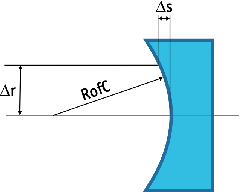
\includegraphics[width = 0.40\textwidth]{Mirrors_scheme1.pdf}\hfill
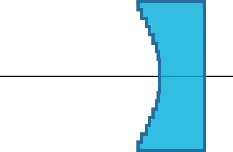
\includegraphics[width = 0.40\textwidth]{Mirrors_scheme2.pdf}\hfill

\vspace*{1cm}

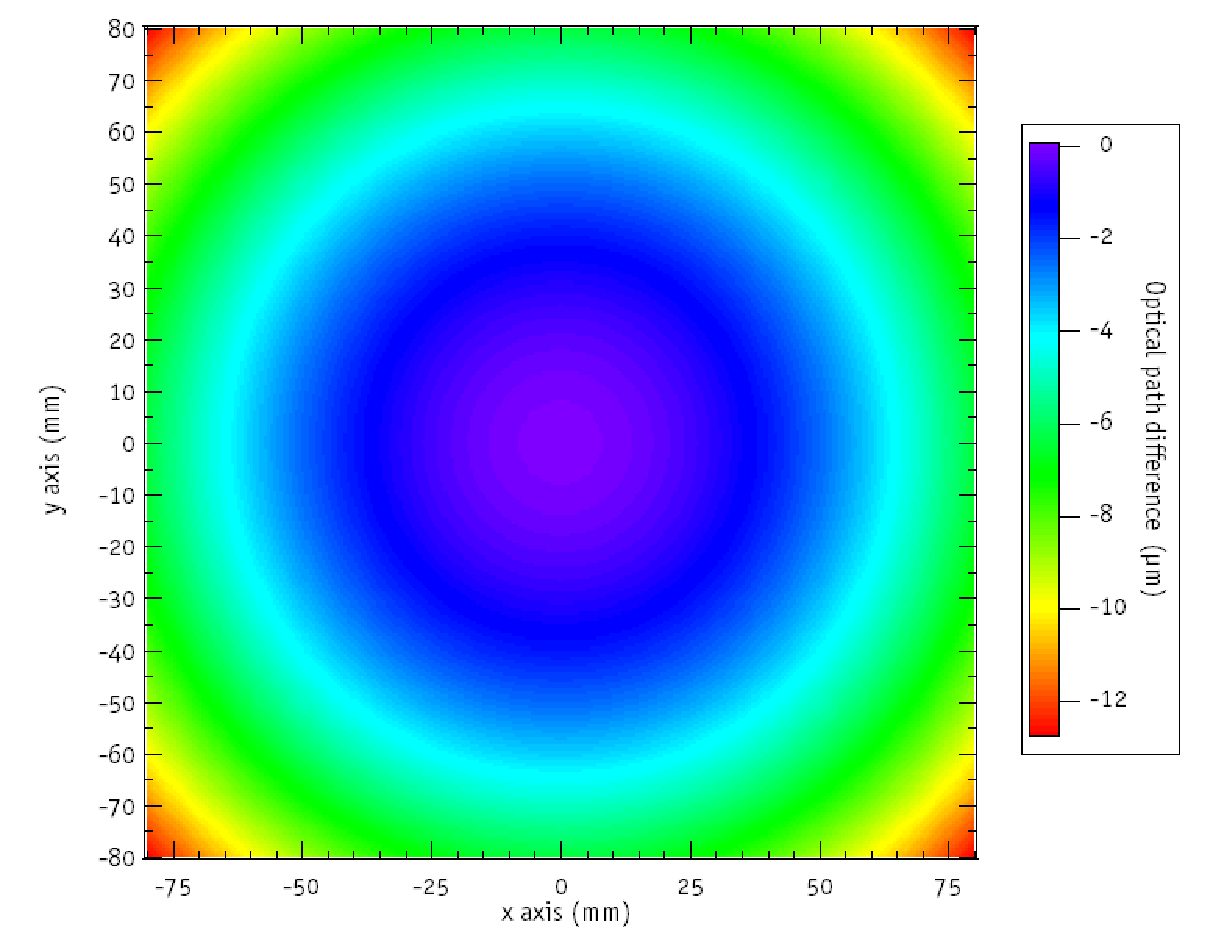
\includegraphics[width = 0.45\textwidth]{Mirror_map_fine.pdf}\hfill
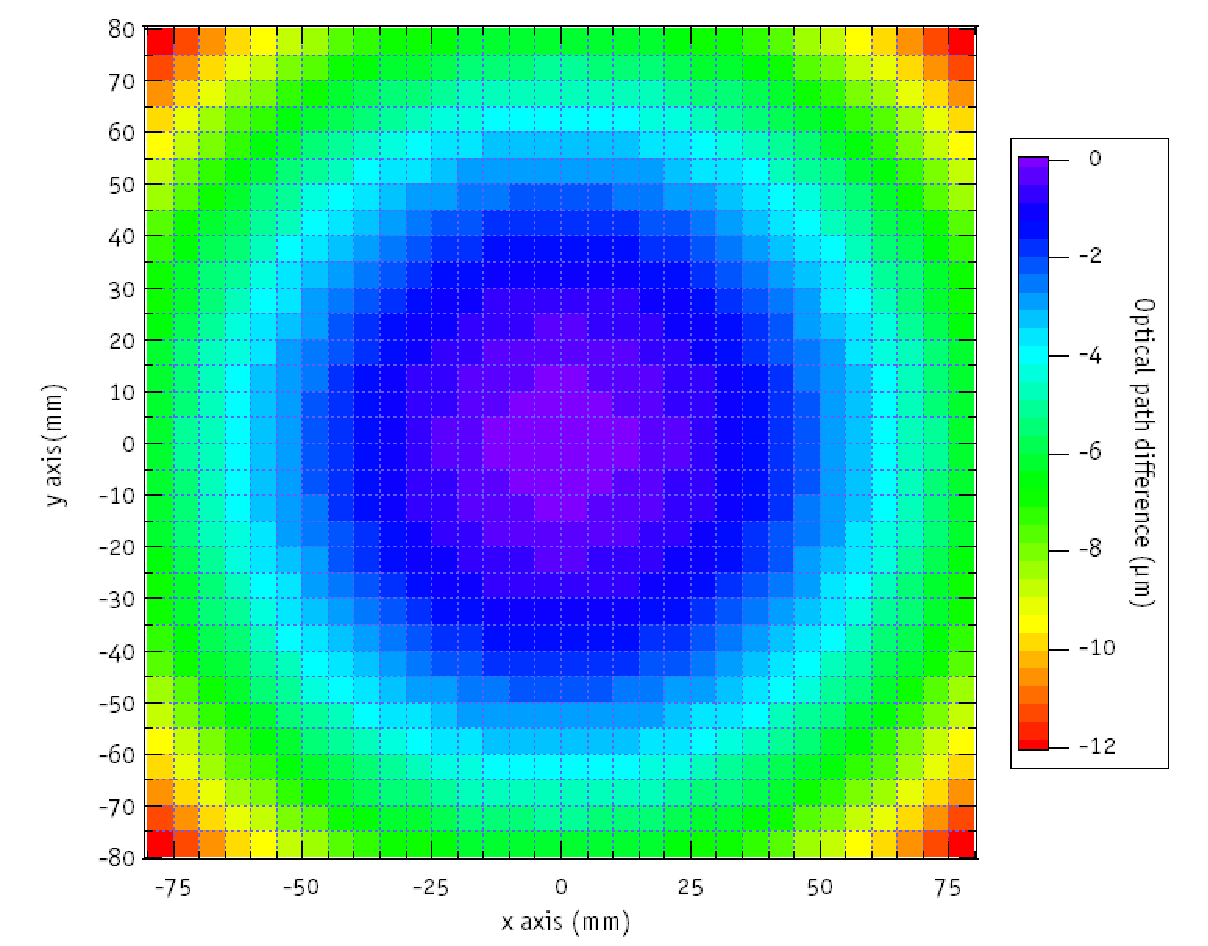
\includegraphics[width = 0.45\textwidth]{Mirror_map.pdf}
\end{center}
\caption{\label{fig4:disct_mirror} Example of the optical path difference induced by 1~km radius of curvature mirror. The optical path difference is simply two times the sagitta of the mirror. The right plot is the left plot discretised on a grid of $32 \times 32$ pixels.}
\end{figure}

Of course since we are using a numerical simulation, the optical path difference representing the mirror has also to be discretized using the same grid as the one used for the laser beam. A discretized optical path difference for a mirror is represented on the right part in the figure \ref{fig4:disct_mirror}.

There is no difficulty to create with Matlab the matrix used to represent the optical path difference induced by a mirror. The value of the optical path as a function of the coordinate $(x,y)$ has previously been shown in equation \ref{eq1:mir_ref_OPN}. The direct Matlab implementation is presented in the listing \ref{lis1:mir1}. By definition in OSCAR a concave mirror has a positive radius of curvature, which means the optical path difference is negative.\\

\begin{lstlisting}[float=htp,caption=The code used to create the mirror matrix \label{lis1:mir1},frame=lines]

% Definition of the mirror radius of curvature in meter
Mirror.RofC = 1000;

% Create mirror grid
Mirror.OPL = zeros(Grid.Num_point,Grid.Num_point,'double');


for m = 1:Grid.Num_point
    for n = 1:Grid.Num_point

        Radius_sqr = (Grid.axis(m)^2+Grid.axis(n)^2);
        Mirror.OPL(m,n) = -2*(Mirror.RofC - sqrt(Mirror.RofC^2 - Radius_sqr));

    end
end
\end{lstlisting}

If the mirror is not perfectly spherical because of thermal lensing effect or because the mirrors are part of a flat beam cavity, we simply have to modify the equation \ref{eq1:mir_ref_OPN} accordingly by adding the known deviation.


\subsection{Lenses}

In OSCAR, we use exactly same procedure as that for mirrors to simulate lenses. The optical path difference induced by the lens is the same as that induced by a mirror whose radius of curvature is two times the focal length of the lens we wish to simulate. The fact that the lens is used in transmission and a mirror in reflection is not relevant in OSCAR. Indeed the evolution of the laser beam confined between two mirrors can always be simulated by the propagation of a laser beam passing through a periodic system of lenses\cite{Kogelnik}.


\subsection{Aperture}

\label{sec1:aperture}

Apertures can be represented by two complementary physical areas: one area transmits integrally the light falling on it whereas the other area blocks integrally the light. Apertures are useful to simulate correctly finite size optics. In OSCAR, the optical path difference representing a mirror is defined over the whole calculation grid independently of the real size of the mirror. To simulate a finite size mirror, we multiply the reflected field by an aperture which has the same diameter as that of the mirror. The aperture simulates the fact that any light falling outside the mirror is lost.\\

Practically, an aperture $A(x,y)$ is represented by matrix of $0$ and $1$. A $0$ at the position $(x,y)$ indicates that the light is blocked and a $1$ indicates that the light is transmitted. An example of a circular aperture is presented in figure \ref{fig1:aperture}. So to simulate the reflection from a finite size mirror, we can include the aperture effect in the previous equation \ref{eq1:mir_ref}:

\begin{equation}
E_o(x,y) = E_i(x,y) \exp{(-j k \Delta OPL(x,y))} A(x,y)
\end{equation}


% 1.5,1.5,3,0.5

\begin{figure}
\begin{center}
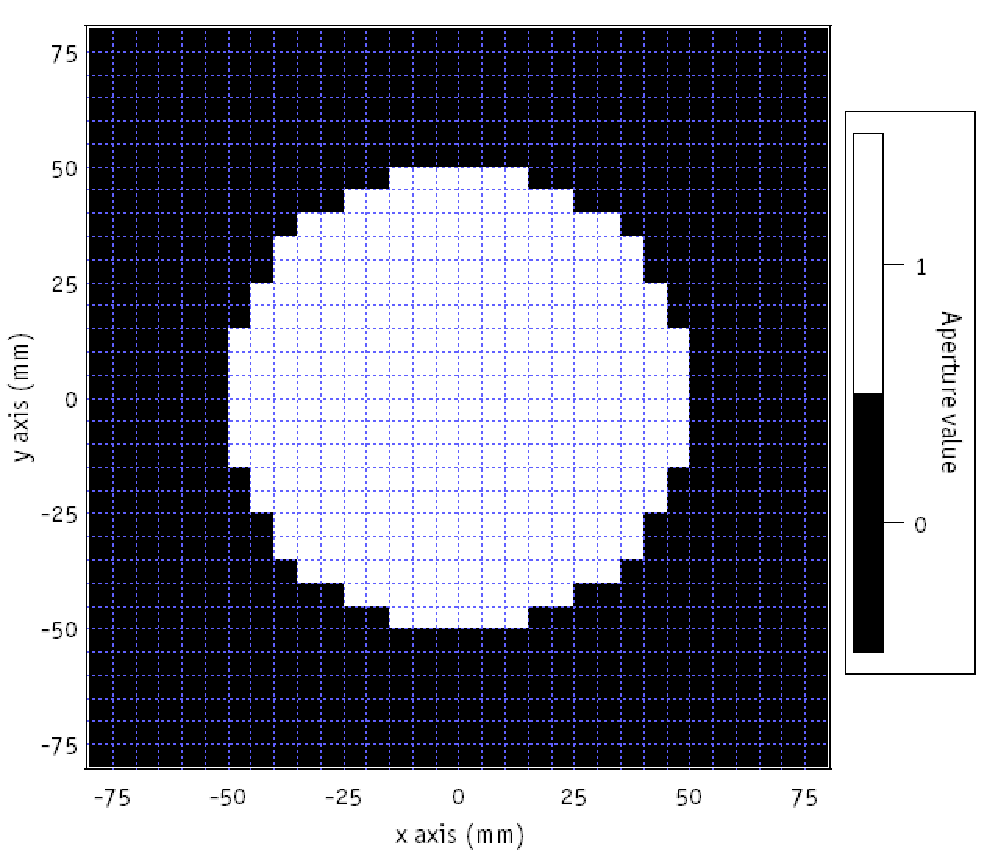
\includegraphics[width = 0.8\textwidth]{Mirror_mask.pdf}
\end{center}
\caption{\label{fig1:aperture} Plot of the 2D matrix representing a circular aperture of diameter 10~cm. The number of points for the grid is $32 \times 32$ points and the physical size of the grid is 16~cm $\times$ 16~cm.}
\end{figure}

As for the optical path induced by the mirror, we can also define a matrix representing the aperture. In the OSCAR code this matrix is called $Mirror.mask$. This matrix is only filled with $0$ and $1$, $1$ when the pixel is inside the mirror and $0$ otherwise. The simple Matlab code to create a circular aperture in OSCAR is described in the listing \ref{lis1:aper1}.\\

\begin{lstlisting}[float=htp,caption=The code used to create a circular aperture \label{lis1:aper1},frame=lines]

% Define aperture diameter in meter
Aperture_diameter = 0.1;

Mirror.mask = zeros(Grid.Num_point,Grid.Num_point,'double');

for m = 1:Grid.Num_point
    for n = 1:Grid.Num_point

        Radius = sqrt(Grid.axis(m)^2+Grid.axis(n)^2);
        if (Radius < Aperture_diameter/2)
            Mirror.mask(m,n) = 1;
        end
    end
end

\end{lstlisting}

\subsection{Code implementation}
\label{sec1:3:5}
To simulate the reflection of an electric field by a mirror (or a transmission through a lens), we define a function called \emph{Propa\_mirror}. The function takes for parameters the input electric field, the optical path difference induced by the mirror and the reflectivity of the mirror as shown in the listing \ref{lis1:refl1} . The output of the function is the electric field after the reflection on the mirror. The function is a direct implementation of the equation \ref{eq1:mir_ref}.

The aperture of the mirror is also included in the reflection however it is not an argument of the function \emph{Propa\_mirror} since we suppose that the mirrors have all the same diameter, so the aperture matrix is constant\footnote{The function can easily be modified if the mirrors have different sizes}. in the function, the reflectivity of the mirror is scalar, which means the reflectivity is homogenous and constant over the mirror surface. The reflectivity of the mirror can also be defined as a matrix if the reflective coating is not perfectly uniform.

\begin{lstlisting}[float=htp,caption=The function used to simulate the reflection of an electric field by a mirror\label{lis1:refl1},frame=lines]

function Output = Propa_mirror(Wave_field, Wave_mirror, reflectivity)

global Mirror;
global Laser;

Output = Wave_field .* exp(i * Wave_mirror*Laser.k_prop) * reflectivity .* Mirror.mask;

\end{lstlisting}


\section{Simulating a Fabry Perot cavity}
\label{sec1.4}

Since we have seen in the two last sections how to propagate a laser beam in free space (section \ref{sec1.2}) and how to simulate the reflection by a mirror (section \ref{sec1.3}), we have all what we need to simulate a Fabry Perot cavity.

A Fabry Perot cavity is usually constituted by two mirrors facing each other. Between these two mirrors, a light field is circulating, bouncing back and forth between the two reflective coatings. One of the main interest of the Fabry Perot is that the optical power of the circulating field can be much higher than the power of the input field. With OSCAR, it is possible for a given input field to calculate the total circulating power, reflected power and transmitted power as well as the spatial profile of all the light fields.\\

The method used by OSCAR to calculate the circulating field in a Fabry Perot cavity is well known for most readers. Indeed, the same method is often used in undergraduate lectures to calculate analytically the circulating field in the cavity\cite{Cav_circ}. OSCAR calculates the circulating field by propagating back and forth the laser beam between the two mirrors and then summing all the fields at one particular plane as shown in figure \ref{fig1:cavity}.

\begin{figure}
\begin{center}
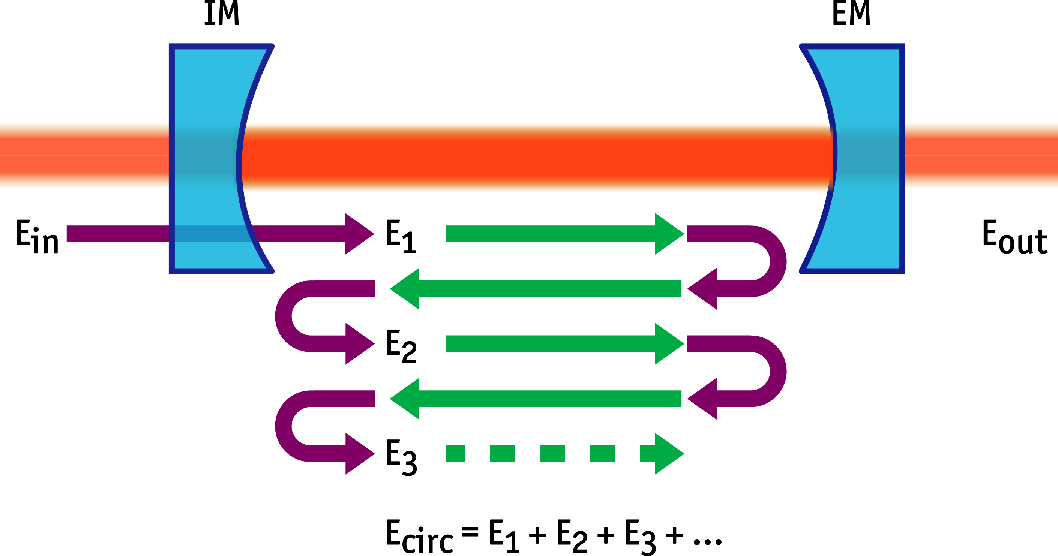
\includegraphics[width = 0.95\textwidth]{C1_cavity.pdf}
\end{center}
\caption{\label{fig1:cavity} Description of the algorithm used in OSCAR to calculate the circulating field in a Fabry Perot cavity. The violet arrows represent a change in phase for the light field which is described by equation \ref{eq1:mir_ref} and the green arrows represent the propagation of the light field using a FFT code. From $E_i$ to $E_{i+1}$, the light field has undergone one round trip in the cavity. IM and EM stand respectively for Input Mirror and End Mirror.}
\end{figure}

In more details, we can write the OSCAR algorithm used to compute the circulating power. Using the notation from the figure \ref{fig1:cavity} the different consecutive steps can be described as:

\begin{enumerate}
  \item Define the cavity parameters as well as the mirror profiles and the input beam.
  \item Propagate the input beam $E_{in}$ through the input mirror . For this purpose the input mirror can assimilated to a lens, so the listing \ref{lis1:refl1} can be used. As a result, we obtain the field $E_1$.
  \item After one round trip in the cavity, the field $E_1$ becomes $E_2$. One round trip in the cavity consists specifically of one propagation through the cavity length using the FFT code, one reflection on the end mirror, another propagation back to the input mirror and then finally a reflection on the input mirror.
  \item Repeat the last operation to create the set of electric field $E_i$.
  \item Then sum all the field $E_i$ to have the cavity circulating power $E_{circ}$. The number of light field $E_i$ to be considered to have an accurate result depends on the finesse of the cavity.
  \item The transmitted field $E_{out}$ is simply the circulating field transmitted through the ETM.
\end{enumerate}

In this above pseudo-code, we did not mention any resonance condition to maximise the circulating power in the cavity. Practically, we should always define the round trip phase shift for the field in the cavity (or a microscopic position shift for the cavity length) before calculating the cavity circulating power. The round trip phase shift allows us to set the cavity to be resonant for the fundamental mode or any other optical modes if necessary. The procedure to find the suitable resonance length is detailed in the next chapter in section \ref{sec2.2}.

\section{Further reading}

In this chapter, only a general and simplistic view of the FFT code has been presented. To have a better understanding of the power and limit of the code some further reading is highly recommended. Here some suggestions:
\begin{itemize}
  \item The thesis from Brett Bochner\cite{Bochner} which programmed one of the first FFT code used by LIGO is a mine of treasures. The chapter two of this thesis about the technical realization of an optical FFT code contains some essential issues to grasp for a successful code, for example how the radius of curvature of the mirror can set an upper limit on the resolution of the grid, the use of aliasing filters or methods to calculate the steady state fields.

  \item Andrew Trigdell wrote also a FFT code in the ANU group. His master thesis may be hard to find but a following article\cite{Tridgell} gives some good insights of the procedures involved in the code.

  \item A wonderful article to understand how to create a simple and robust FFT code to simulate high finesse cavity has been written by Partha Saha. The explanation how to calculate the steady state cavity circulating field is crystal clear and very elegant (however the end of the article may appear a little bit more obscure at the first reading).

  \item Technics to build a FFT code (and some other optical numerical codes) can be found in the recent thesis of Juri Agresti\cite{Juri}. This thesis is also an excellent example about how to deal with non spherical mirror.

 \item One of the first article describing how to use a FFT to calculate the eigen modes of a cavity by Gordon and Li\cite{Gordon}. Although the article is 40 years old, all the modern FFT program are still based on the fundamental method explained in this paper.

\end{itemize}







